\documentclass[dvipdfmx]{jsarticle}

\usepackage{ascmac}
\usepackage{url}
\usepackage[dvipdfmx]{hyperref}
\usepackage{pxjahyper}
\usepackage[dvipdfmx]{graphicx}
\usepackage{float}
\usepackage{listings,jlisting}

\hypersetup{
  colorlinks=true,
  urlcolor=cyan,
  linkcolor=black
}

\lstset{
  basicstyle={\ttfamily},
  identifierstyle={\small},
  commentstyle={\smallitshape},
  keywordstyle={\small\bfseries},
  ndkeywordstyle={\small},
  stringstyle={\small\ttfamily},
  frame={tb},
  breaklines=true,
  columns=[l]{fullflexible},
  numbers=left,
  xrightmargin=0zw,
  xleftmargin=3zw,
  numberstyle={\scriptsize},
  stepnumber=1,
  numbersep=1zw,
  lineskip=-0.5ex
}


\begin{document}

\section{実験目的・課題}

Socket通信を行いクライアントと通信し、
クライアントから入力された成績情報を
記録するサーバプログラムを作成する。

作成するサーバーの要件
\begin{itemize}
  \item サーバープログラムとクライアントプログラムをわけて作成
  \item 接続したクライアントは何度でもメッセージのやり取りが出来る
  \item 新しく成績情報と登録できる
  \item 登録された成績情報を記録できる
  \item 今までに登録された成績情報を閲覧できる
  \item 名前か番号で検索できる
  \item 入力にエラーがある場合は通知できる
  \item 名前と番号は重複登録はできない
\end{itemize}


\section{実装方法}
Javaで複数のプログラム間でデータのやり取りを行うときは、
Socket通信というものを用いて通信を行う。

ここに、2つのプログラムがあり、この2つで通信を行いたいとき、
一方を「サーバー」もう一方を「クライアント」として話をする。
サーバーとクライアントは最初、何のつながりも持っていない。
ここで、サーバー側がServerSocketクラスをインスタンス化し、
その際に受け取ったポート番号の監視を始める。
次に、クライアント側でSocketクラスにサーバー名とポート番号を渡し
インスタンス化する際にサーバーに接続要求が送られる。
サーバー側ではこのSocketによる接続要求をacceptメソッドによって
受け取り、これで2つのプログラム間の接続が完了する。

\subsection{全体の方針}
今回の成績情報サーバーの作成では、サーバーとクライアントが交互に
入出力を行うことにする。
サーバーからクライアントにメッセージを送信、
それを受け取ったクライアントがそのメッセージを標準出力に出力、
それを見たユーザーがそれに対する応答をキーボードから入力する。
その入力をクライアントよりサーバーに送信し、
その入力を受けてサーバーで処理を行う。
このまとまりを処理のひとまとまりとして扱い、
これを繰り返すことで成績情報サーバーを作成する。
この処理の例を図\ref{example1}に示す。
\begin{figure}[H]
  \centering
  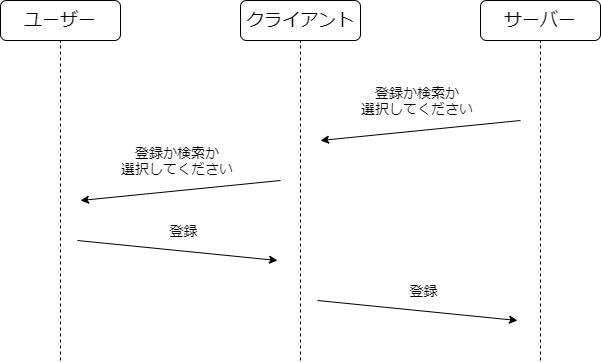
\includegraphics[width=0.7\hsize]{../pic/1.png}
  \caption{サーバーとクライアントの入出力例}
  \label{example1}
\end{figure}

クライアントプログラムでは、処理のひとまとまりを順に処理すればよいので
ソケット入力、標準出力、標準入力、ソケット出力を順に1回だけ行うコードを
whileで囲い何度もループさせればよい。

サーバープログラムでは、サーバーの要件に従い、
成績情報の登録、検索、閲覧ができるものを作成する。

\subsection{情報の記録}
今回作成するプログラムは登録された情報を外部ファイルに書き込み保存し、
次回サーバー起動時にそれを読み込み登録済み情報として保持することが出来るようにする。
成績情報が書かれたファイルからの入力は「実験4 ファイルからの入力と正規表現」
で作成したプログラムのものを改変して使用する。
出力ファイルへの書き込みはプログラム終了時に行い、
Number,Name,Scoreをタブ区切りで出力する。

プログラム中でseisekiクラスのデータの保持にはArrayListではなく
TreeMapを使用する。
TreeMap \textless K,V\textgreater は型Kのキーによって型Vの値にアクセスすることができるデータ構造である。
型Kによって比較する赤黒木によって実装されており、
要素数Nのとき、要素の検索、挿入、削除がlog(n)時間で行うことができるため、
検索の面でArrayListより優れていると判断し、これを採用した。

また、成績情報の入力において番号がバラバラに入力される可能性があるが、
TreeMapでデータを保存しておけばプログラムの最後に出力するときにキーの
昇順で成績情報を得られるので、
データの閲覧時にわかりやすさが向上することが見込める。

\subsection{登録}
成績情報の登録にはNumber,Name,Scoreが必要である。
今回はこれを一度に入力してもらうのではなく、それぞれについて
クエリを投げてそれに回答してもらう形式にする。
こうしなかった場合、例えばNumberとNameの区切り文字を
どうするかという事も決めなければならなくなるうえ、
入力にミスが含まれる可能性が高くなると考えられる。
こうしてNumberを表す文字列、Nameを表す文字列、...を得られる。
次にそれに区切り文字を付け一つの文字列になるよう連結する。
このようにして得られた文字列が正規表現に
マッチすれば入力をseisekiクラスに変換できる。

seisekiクラスに変換できたとしても、すぐに登録はできず、
名前と番号が今までに登録されたものと重複していないか確認しなければならない。
これは、名前、番号をそれぞれキーとした2つのTreeMapを用意しておいて
それぞれでcontainsKeyメソッドで確認すればよい。

入力が正規表現にマッチし、今までと重複したものでもなければ新たに
TreeMapに挿入する。

\subsection{検索}
名前で検索する場合は名前をキーとしたTreeMap \textless String,seiseki\textgreater で
検索を行い、キーとして名前が存在すればその名前でputすれば良い。

番号で検索する場合は番号をキーとしたTreeMap \textless Integer,seiseki\textgreater で
検索を行い、キーとして番号が存在すればその番号でputすれば良い。

\subsection{閲覧}
番号をキーとしたTreeMapのvaluesメソッドを使い、番号の昇順にならんだ
seisekiクラスの集合を得る。それぞれに対して文字数が
図\ref{seiseki_format}のようにフォーマットした文字列を送信する。
\begin{figure}[H]
  \centering
  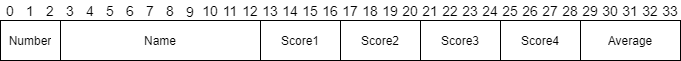
\includegraphics[width=0.9\hsize]{../pic/seiseki_format.png}
  \caption{成績クラスの文字列フォーマット}
  \label{seiseki_format}
\end{figure}

この時だけ他の通信の時と違い、1行だけでなくデータ数行分送信を行う。
クライアント側では、通常1行受け取る処理しかしていないため、
データ一覧を要求したときだけif文を使い複数行の入力に対応している。

\subsection{サーバーのマルチスレッド化}

JavaではThreadクラスの継承やRunnableインターフェースを実装することで
プログラムを並列実行させることが出来る。
ソースコード\ref{mt1}を実行した結果を図\ref{mt_r_1},\ref{mt_r_2}
に示す。
\begin{lstlisting}[caption=マルチスレッドの例,label=mt1]
  public class Main extends Thread {
    public static void main(String[] args){
      Thread t1 = new Main();
      Thread t2 = new Main();
      t1.start();
      t2.start();
    }
    public void run() {
      for (int i = 0; i < 5; ++i)
        System.out.println(getName() + " : " + i);
    }
  }  
\end{lstlisting}
\begin{figure}[H]
  \begin{minipage}{0.5\hsize}
    \begin{center}
      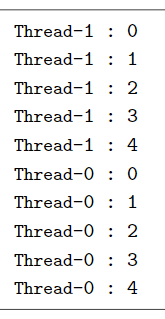
\includegraphics[width=0.4\hsize]{../pic/3_1.png}
    \end{center}
    \caption{2回目の実行結果}
    \label{mt_r_1}
  \end{minipage}
  \begin{minipage}{0.5\hsize}
    \begin{center}
      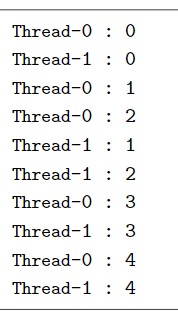
\includegraphics[width=0.4\hsize]{../pic/3_2.png}
    \end{center}
    \caption{2回目の実行結果}
    \label{mt_r_2}
  \end{minipage}
\end{figure}

図\ref{mt_r_1}と\ref{mt_r_2}で実行結果が異なっていることがわかる。
このようにして並列実行では同時にプログラムを実行することが出来る。
ソースコード\ref{mt1}の5,6行目のstartメソッドがThreadの実行を表しており、
オーバーライドされたrunメソッドが実行される。
runメソッドではgetNameメソッドによりスレッド名を取得しそれとともに0から4までの
数字を表示するだけのプログラムを実行させている。
図\ref{mt_r_1},\ref{mt_r_2}ともにThread-0だけ、Thread-1だけ、で見てみると
0から1,2,3,4の順に表示されていることから、run内の処理は
逐次実行されているとわかる。

これによって、サーバープログラムを並列実行させることで、
クライアントが複数起動してもすべてに対応して情報をアップデート
できるプログラムを作成する。

次に、変数の共有についてソースコード\ref{mt2}に示すものを実行すると、
"asdf1234"と表示される。
本来これに期待される動作は"asdf"に"1234"を10回連接したものである。
しかし、各スレッドでString型の変数sは共有されていないため、
1回だけ"1234"を連接したものが出力されてしまう。
サーバープログラムではプログラムの動作中は
成績情報をTreeMapによって管理しているため、
複数のスレッドでそれぞれに追加された成績情報が共有されなければ
重複登録が起こってしまう可能性が高いため、これは許容できない。

\begin{lstlisting}[caption=マルチスレッドの例2,label=mt2]
  public class Main {
    public static void main(String[] args) {
      String s = "asdf";
      hoge fuga = new hoge(s);
      Thread t[] = new Thread[10];
      for (int i = 0; i < 10; ++i) t[i] = new Thread(fuga);
      for (int i = 0; i < 10; ++i) t[i].start();
      for (int i = 0; i < 10; ++i)
        try {
          t[i].join();
        } catch (InterruptedException e) {
          e.printStackTrace();
        }
      System.out.println(fuga.getStr());
    }
  }
  class hoge implements Runnable {
    private String str;
    public hoge(String s) {
      this.str = s;
    }
    public void run() {
      this.str += "1234";
    }
    public String getStr() {
      return this.str;
    }
  }
\end{lstlisting}

これは、Stringがスレッドセーフなクラスではないためである。
スレッドセーフとはあるプログラムを並列実行しても問題がないことである。
スレッドセーフではないとは、あるスレッドで変更した共有データが
他のスレッドによって上書きされてしまう可能性があることである。

ここで、CollectionsクラスのsynchronizedSortedMapメソッドを使うことで
スレッドセーフなソート・マップを使用することが出来る。
今回はこれを使用してスレッドセーフなサーバークラスを作成した。

\section{結果と考察}

成績情報に表\ref{out0}の情報が出力ファイルに書き込まれているところから、
"7 Mia 74 64 62 72"を追加するときのサーバーのログをソースコード\ref{add_1}
に示す。
\begin{table}[H]
  \begin{tabular}{cccccc}
    Number & Name    & Score1 & Score2 & Score3 & Score4 \\
    1      & Michael & 75     & 86     & 89     & 31     \\
    2      & Emma    & 74     & 63     & 70     & 48     \\
    3      & Hannah  & 73     & 45     & 82     & 31     \\
    4      & Emily   & 40     & 30     & 49     & 48     \\
    5      & Daniel  & 46     & 59     & 47     & 70     \\
    6      & Oliver  & 59     & 26     & 61     & 44
  \end{tabular}
  \centering
  \caption{事前に書き込まれている成績情報}
  \label{out0}
\end{table}

\begin{lstlisting}[caption=成績情報追加1,label=add_1]
  Thread-0:send[select search,add,list : ]
  Thread-0:recv[add]
  Thread-0:send[Number : ]
  Thread-0:recv[7]
  Thread-0:send[  Name : ]
  Thread-0:recv[Mia]
  Thread-0:send[Score1 : ]
  Thread-0:recv[74]
  Thread-0:send[Score2 : ]
  Thread-0:recv[64]
  Thread-0:send[Score3 : ]
  Thread-0:recv[62]
  Thread-0:send[Score4 : ]
  Thread-0:recv[72]
  Thread-0:send[added data "  7       Mia  74  64  62  72 68.0"  (enter to next)]
  Thread-0:recv[]
\end{lstlisting}

ログ出力の1行は3つの部分からなり、最初に通信しているスレッド名、
次に送信(send)か、受信(receive)か、最後に送受信された文字列を出力している。
このときは1つのクライアントしか起動していないのでスレッド名は同じである。
最初に定めた通信の手順に従い、送信と受信を交互に行っている。
一番最初に送信した文字列によってデータの追加か検索か、一覧の出力を選択してもらい、
それ以降は各クエリについての手順に従っている。
成績の追加クエリでは、Number,Name,Scoreのそれぞれについて問いかけを行い回答を
受け取り、seisekiクラスにパースしてデータを保存している。
このときに登録されたMiaの情報はプログラム内で保持されるのみで出力ファイルに
出力はされていない。

次に、名前か番号が重複している入力、得点にエラーがある入力をしたときの出力を
ソースコード\ref{out2}に示す。
\begin{lstlisting}[caption=不正な成績追加入力,label=out2]
  Thread-0:send[select search,add,list : ]
  Thread-0:recv[add]
  Thread-0:send[Number : ]
  Thread-0:recv[8]
  Thread-0:send[  Name : ]
  Thread-0:recv[Mia]
  Thread-0:send[Score1 : ]
  Thread-0:recv[1]
  Thread-0:send[Score2 : ]
  Thread-0:recv[1]
  Thread-0:send[Score3 : ]
  Thread-0:recv[1]
  Thread-0:send[Score4 : ]
  Thread-0:recv[1]
  Thread-0:send[duplication name  (enter to next)]
  Thread-0:recv[]
  Thread-0:send[select search,add,list : ]
  Thread-0:recv[add]
  Thread-0:send[Number : ]
  Thread-0:recv[2]
  Thread-0:send[  Name : ]
  Thread-0:recv[Luna]
  Thread-0:send[Score1 : ]
  Thread-0:recv[52]
  Thread-0:send[Score2 : ]
  Thread-0:recv[72]
  Thread-0:send[Score3 : ]
  Thread-0:recv[57]
  Thread-0:send[Score4 : ]
  Thread-0:recv[56]
  Thread-0:send[duplication number  (enter to next)]
  Thread-0:recv[]
  Thread-0:send[select search,add,list : ]
  Thread-0:recv[add]
  Thread-0:send[Number : ]
  Thread-0:recv[8]
  Thread-0:send[  Name : ]
  Thread-0:recv[James]
  Thread-0:send[Score1 : ]
  Thread-0:recv[86]
  Thread-0:send[Score2 : ]
  Thread-0:recv[611]
  Thread-0:send[Score3 : ]
  Thread-0:recv[51]
  Thread-0:send[Score4 : ]
  Thread-0:recv[78]
  Thread-0:send[invalid seiseki input  (enter to next)]
  Thread-0:recv[]  
\end{lstlisting}

1つ目は、"8 Mia 1 1 1 1"と入力している。これはMiaという名前が先に
登録したものと同じため登録できない。
次に、"2 Luna 52 72 57 56"と入力しているがこれは最初からファイルに
入力してあった場号なので登録できない。
最後に、"8 James 86 611 51 78"とい入力している、これは名前も番号も
重複はしていないが点数が611点の入力があるため正規表現にマッチせず、
入力にエラーありと判断される。

次に、2つ目のクライアントを起動して2つのクライアントで
同じデータを追加しようとしたときのサーバーのログ出力を
ソースコード\ref{out3}に示す。

\begin{lstlisting}[caption=別のクライアントによる登録,label=out3]
  Thread-0:send[select search,add,list : ]
  new Thread
  Thread-1:send[select search,add,list : ]
  Thread-1:recv[add]
  Thread-1:send[Number : ]
  Thread-1:recv[10]
  Thread-1:send[  Name : ]
  Thread-1:recv[Luna]
  Thread-1:send[Score1 : ]
  Thread-1:recv[52]
  Thread-1:send[Score2 : ]
  Thread-1:recv[72]
  Thread-1:send[Score3 : ]
  Thread-1:recv[57]
  Thread-1:send[Score4 : ]
  Thread-1:recv[56]
  Thread-1:send[added data " 10      Luna  52  72  57  56 59.3"  (enter to next)]
  Thread-1:recv[]
  Thread-1:send[select search,add,list : ]
  Thread-0:recv[add]
  Thread-0:send[Number : ]
  Thread-0:recv[10]
  Thread-0:send[  Name : ]
  Thread-0:recv[Luna]
  Thread-0:send[Score1 : ]
  Thread-0:recv[52]
  Thread-0:send[Score2 : ]
  Thread-0:recv[72]
  Thread-0:send[Score3 : ]
  Thread-0:recv[57]
  Thread-0:send[Score4 : ]
  Thread-0:recv[56]
  Thread-0:send[duplication name  (enter to next)]
  Thread-0:recv[]
\end{lstlisting}

1行目のセレクトクエリがスレッド0によって送られているが
それに接続しているクライアントが何らかの入力をするまでは
何もできないため待機している。
2行目の"new thread"というのはメイン関数内で新たにポートに
接続要求をしてきたクライアントがいたため新しくserver.acceptをし、
別のソケットで新しいスレッドを開始したことを通知するものである。
新しく開始したスレッド1によって"10 Luna 52 72 57 56"を追加し、
その後、同じデータをスレッド0によって追加しようとしている。
スレッド0によって追加しようとしたときは、データの重複のため、
登録できていない。このことから、
複数のスレッドで成績データを管理しているTreeMapが同期されていることがわかる。

次に、検索クエリでの動作をソースコード\ref{out4}に示す。
このときの成績データを表\ref{data2}に示す。
\begin{table}[H]
  \begin{tabular}{cccccc}
    Number  Name  Score1  Score2  Score3  Score4
    1	Michael	75	86	89	31
    2	Emma	74	63	70	48
    3	Hannah	73	45	82	31
    4	Emily	40	30	49	48
    5	Daniel	46	59	47	70
    6	Oliver	59	26	61	44
    7	Mia	74	64	62	72
    10	Luna	52	72	57	56
  \end{tabular}
  \centering
  \caption{検索をするときのデータ}
  \label{data2}
\end{table}
\begin{lstlisting}[caption=検索クエリ,label=out4]
  Thread-0:send[select search,add,list : ]
  Thread-0:recv[search]
  Thread-0:send[select Number,Name : ]
  Thread-0:recv[name]
  Thread-0:send[enter name : ]
  Thread-0:recv[Mason]
  Thread-0:send[not found  (enter to next)]
  Thread-0:recv[]
  Thread-0:send[select search,add,list : ]
  Thread-0:recv[search]
  Thread-0:send[select Number,Name : ]
  Thread-0:recv[name]
  Thread-0:send[enter name : ]
  Thread-0:recv[Luna]
  Thread-0:send[ 10      Luna  52  72  57  56 59.3  (enter to next)]
  Thread-0:recv[]
  Thread-0:send[select search,add,list : ]
  Thread-0:recv[search]
  Thread-0:send[select Number,Name : ]
  Thread-0:recv[number]
  Thread-0:send[enter number : ]
  Thread-0:recv[111]
  Thread-0:send[not found  (enter to next)]
  Thread-0:recv[]
  Thread-0:send[select search,add,list : ]
  Thread-0:recv[search]
  Thread-0:send[select Number,Name : ]
  Thread-0:recv[number]
  Thread-0:send[enter number : ]
  Thread-0:recv[1]
  Thread-0:send[  1   Michael  75  86  89  31 70.3  (enter to next)]
  Thread-0:recv[]  
\end{lstlisting}

存在しない番号、名前で検索しようとしたときは"not found"となっていて、
存在する番号、名前で検索したときは、Number,Name,Score,Acerageが
表示されていることがわかる。

成績のデータを追加するときの重複判定、実際に追加すること、
検索の時の存在判定はいずれもデータ数をNとして$θ(logN)$で
実現されている。

\begin{thebibliography}{10}
  \bibitem{1} Javaプログラムにおける通信のしくみを理解する

  \url{https://crew-lab.sfc.keio.ac.jp/lectures/2000s_mmb/JavaLectures/Lecture8/Lec8-1.html}
\end{thebibliography}
\end{document}